\documentclass[12pt]{article}
\usepackage{class/sbc-template}
\usepackage{graphicx,url}
\usepackage[utf8]{inputenc}
\usepackage[brazil]{babel}
\usepackage{color}
\usepackage{listings}

%%%%%%%%%%%%%%%%%%%%%%%%%%%%%%%%%%%%%%%%%%%%%%%%%%%%
% C O N F I G U R A Ç Õ E S  D O S   C Ó D I G O S %
%%%%%%%%%%%%%%%%%%%%%%%%%%%%%%%%%%%%%%%%%%%%%%%%%%%%

\lstset{
	numbers=left,
	stepnumber=1,
	firstnumber=1,
	numberstyle=\tiny,
	extendedchars=true,
	breaklines=true,
	frame=single,
	showstringspaces=false,
	xleftmargin=2.5em,
	framexleftmargin=2em,
	basicstyle=\small,
}

\renewcommand{\lstlistingname}{Código}
\renewcommand{\lstlistlistingname}{Lista de Códigos}

\sloppy

\title{Aprendizagem de Máquina (2020/Período Especial) - Impactos da Representação}

\author{Diogo C. T. Batista\inst{1}}

\address{Universidade Federal do Paraná (UFPR)\\
	Curitiba -- Paraná -- Brasil
	\email{diogo@diogocezar.com}
	}

\begin{document}

\maketitle

\section{Representação}

Esta atividade laboratorial tem como objetivo a investigação exploratória de um algorítmo para a classificação de imagens. As imagens analisadas são representações manuscritas de dígitos de 10 categorias diferentes, que representam os número decimais $0,1,2,3,4,5,6,7,8,9$. A Figura \ref{fig:image_1_digits} demonstra alguns exemplos das imagens que devem ser classificadas.

\begin{figure}[!htb]
  \centering
  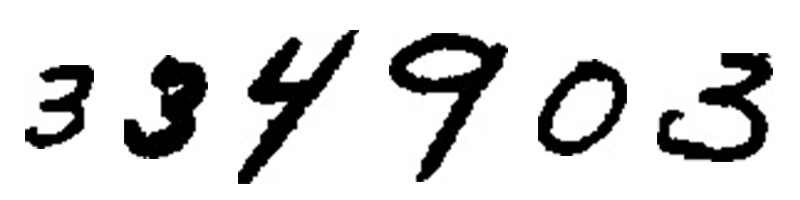
\includegraphics[width=15em]{images/image_1_digits.jpg}
  \caption{Dígitos a serem classificados}
  \label{fig:image_1_digits}
\end{figure}

Além das figuras, um arquivo de texto rotula cada uma das imagens, classificando-a em alguma categoria. Como no exemplo do Código \ref{code:exemplo_rotulos}.

\begin{lstlisting}[caption={Exemplo dos Rótulos},captionpos=b,frame=single,label={code:exemplo_rotulos}]
data/cdf0361_07_13_0.jpg 0
data/cdf1697_45_29_0.jpg 0
data/cdf0872_30_6_1.jpg 0
data/cdf0371_24_4_0.jpg 0
data/cdf1539_20_17_2.jpg 0
\end{lstlisting}

A atividade se iniciou com base na implementação do programa \textit{digits.py} que extrai uma representação bem simples de cada uma das imagens. Para cada imagem, se gera uma nova imagem no tamanho de $10 x 20$. E para cada pixel, verifica-se o seu valor de intensidade; se esse valor for maior que $128$, a característica é igual a $1$, caso contrário $0$.

Neste ponto, notou-se a possibilidade da primeira exploração. Além do tamanho inicial proposto, uma adaptação no algorítmo realizou uma análise em toda a base de imagens, obtendo outras dimensões para verificação. As estratégias adotadas foram:

\begin{enumerate}
  \item Obter a média entre todas alturas e larguras;
  \item Obter a mediana entre todas alturas e larguras;
  \item Obter os valores máximos entre alturas e larguras;
\end{enumerate}

Após análise dos resultados, notou-se que a média e a mediana retornaram resultados muitos similares, por isso, optou-se apenas pela utilização da mediana. A Tabela \ref{tab:estrategias_representacao} mostra as coleções utilizadas nos experimentos. Além da médiana (med\_x, med\_y), os maiores valores encontrados para as dimensões (max\_x e max\_y) também foram considerados. E ainda, empiramente os valores de $x,y$ como $[20,40]$ e $[30,60]$.

\begin{table}[!htb]
  \centering
  \begin{tabular}{|c|c|c|c|c|c|}
  \hline
  \textbf{X\_Source} & \textbf{Y\_Source} & \textbf{X} & \textbf{Y} & \textbf{File Size} & \textbf{Execution Time (s)} \\ \hline
  20                 & 10                 & 20         & 10         & 2180534            & 1.57                    \\ \hline
  40                 & 20                 & 40         & 20         & 9377970            & 4.84                    \\ \hline
  60                 & 30                 & 60         & 30         & 22978779           & 11.04                   \\ \hline
  med\_x             & med\_y             & 36         & 46         & 20962221           & 10.54                   \\ \hline
  max\_x             & max\_y             & 99         & 81         & 110050116          & 46.63                   \\ \hline
  \end{tabular}
  \caption{Estratégias de representação}
  \label{tab:estrategias_representacao}
\end{table}

Para automatização da geração das representações, foram criadas adaptações no código para que fosse possível utilizar como entrada um arquivo do tipo JSON demonstrado no Código \ref{code:json_representacao}:

\begin{lstlisting}[caption={JSON para representações},captionpos=b,frame=single,label={code:json_representacao}]
[
  {
    "data": "features_20_10",
    "x": 20,
    "y": 10
  },
  ...
]
\end{lstlisting}

Neste JSON, \textit{data} é o nome da coleção de representações, $x$ e $y$ podem ser valores fixos ou terem os valores para obtenção dinâmica de: \textit{avg\_x, avg\_y, med\_x, med\_y, max\_x, max\_y}.

\section{Experimentos}

Assim como na adaptação do primeiro algoritmo, um sistema de entrada JSON possibilitou a variação de combinações para análise de diferentes resultados.

\begin{itemize}
  \item O arquivo de representação fonte; as variações testadas foram: [features\_10\_20, features\_20\_40, features\_30\_60, features\_46\_36, features\_81\_99]
  \item Ativar ou desativar a normalização; as variações testadas foram: [0,1]
  \item Alterar o tipo de distância; as variações testadas foram: [eucledian, manhattan]
  \item Alterar o K; as variações testadas foram: [1,3,4,5,6,7,8,9,10,11,12,13]. Foram considerados os $K$ pares, apenas para efeito de comparações, sabendo-se se sua ineficiência por natureza.
\end{itemize}

\newpage

O Código \ref{code:json_experimentos} mostra as opções de entrada para o algorítmo, podendo variar:

\begin{lstlisting}[caption={JSON para experimentos},captionpos=b,frame=single,label={code:json_experimentos}]
[
  {
    "data": "features_20_10",
    "normalized": 0,
    "distance": "euclidean",
    "k": 1
  },
  ...
]
\end{lstlisting}

\section{Resultados}

Foram realizadas \textit{240} execuções para as variações listadas anteriormente. Os \textit{20} melhores resultados (ordenados por Acurácia e F1Score) estão detalhados na Tabela \ref{tab:resultados_melhores}. Já os 20 piores resultados (ordenados por Acurácia e F1Score) estão detalhados na Tabela \ref{tab:resultados_piores}.

Pode-se observar que os melhores resultados foram obtidos a partir das representações que consideraram as \textit{maiores} alturas e larguras das imagens (99x81). Isso acontece pois, no momento em que se realiza a compressão das imagens, características são perdidas. O melhor resultado teve a \textit{Acurácia} de $0,928$ e o \textit{F1Score} de $0,929$ demorando $2.743$ segundos para execução completa.

Já para nos piores resultados, nota-se que foram obtidos na variação de K: $K=13$, $K=12$, $K=10$. Quanto ao $K$ para os melhores resultados, percebe-se que foram obtidos com $K=1$, seguido de $K=3$ e $K=5$. Isso mostra que a distribuição possui uma particularidade interessante, na qual ao se comparar apenas os vizinhos mais próximos se consegue um melhor resultado. Como já esperado, para os resultados nos quais $K$ tinha um valor par, seus resultados foram menos eficientes.

Em outra análise, a estratégia de obter as médias das alturas e larguras também apresentaram resultados significativos (imagens de dimensão $36x46$), mas ficaram abaixo dos resultados da estratégia empírica que utiliza imagens $60x30$. O destaque é para o tempo de execução em \textit{features\_60\_30}, que conseguiu-se uma Acurácia de $0,925$ e o F1Score de $0,926$ demorando apenas $203$ segundos para execução completa.

As normalizações não parecem fazer muita diferença nos resultados, pois estes já se encontram bem distribuídos.

Em geral a alteração da estratégia de medição das distâncias (\textit{euclidean} e \textit{manhattan}) não influenciaram em uma melhoria da \textit{Acurácia} ou do \textit{F1Score}. O que se pode notar, foi que nos testes executados a estratégia \textit{manhattan} impacta negativamente no tempo de execução.

\begin{table}[!htb]
  \centering
  \begin{tabular}{|c|c|c|c|c|c|c|}
  \hline
  \textbf{Experiment} & \textbf{Normalized} & \textbf{Distance} & \textbf{K} & \textbf{Accuracy} & \textbf{F1Score} & \textbf{Execution Time (s)} \\ \hline
  features\_99\_81    & 0                   & euclidean         & 1          & 0,928             & 0,929            & 2.743                       \\ \hline
  features\_99\_81    & 0                   & manhattan         & 1          & 0,928             & 0,929            & 3.161                       \\ \hline
  features\_99\_81    & 1                   & euclidean         & 1          & 0,928             & 0,929            & 3.550                       \\ \hline
  features\_99\_81    & 1                   & manhattan         & 1          & 0,928             & 0,929            & 3.961                       \\ \hline
  features\_60\_30    & 0                   & euclidean         & 1          & 0,925             & 0,926            & 203                         \\ \hline
  features\_60\_30    & 0                   & manhattan         & 1          & 0,925             & 0,926            & 293                         \\ \hline
  features\_60\_30    & 1                   & euclidean         & 1          & 0,925             & 0,926            & 380                         \\ \hline
  features\_60\_30    & 1                   & manhattan         & 1          & 0,925             & 0,926            & 471                         \\ \hline
  features\_36\_46    & 0                   & euclidean         & 1          & 0,923             & 0,924            & 558                         \\ \hline
  features\_36\_46    & 0                   & manhattan         & 1          & 0,923             & 0,924            & 641                         \\ \hline
  features\_36\_46    & 1                   & euclidean         & 1          & 0,923             & 0,924            & 720                         \\ \hline
  features\_36\_46    & 1                   & manhattan         & 1          & 0,923             & 0,924            & 804                         \\ \hline
  features\_36\_46    & 0                   & euclidean         & 3          & 0,919             & 0,921            & 565                         \\ \hline
  features\_36\_46    & 0                   & manhattan         & 3          & 0,919             & 0,921            & 647                         \\ \hline
  features\_36\_46    & 1                   & euclidean         & 3          & 0,919             & 0,921            & 727                         \\ \hline
  features\_36\_46    & 1                   & manhattan         & 3          & 0,919             & 0,921            & 811                         \\ \hline
  features\_99\_81    & 0                   & euclidean         & 3          & 0,919             & 0,921            & 2.778                       \\ \hline
  features\_99\_81    & 0                   & manhattan         & 3          & 0,919             & 0,921            & 3.193                       \\ \hline
  features\_99\_81    & 1                   & euclidean         & 3          & 0,919             & 0,921            & 3.584                       \\ \hline
  features\_99\_81    & 1                   & manhattan         & 3          & 0,919             & 0,921            & 3.992                       \\ \hline
  \end{tabular}
  \caption{Melhores Resultados}
  \label{tab:resultados_melhores}
\end{table}

\begin{table}[!htb]
  \centering
  \begin{tabular}{|c|c|c|c|c|c|c|}
  \hline
  \textbf{Experiment} & \textbf{Normalized} & \textbf{Distance} & \textbf{K} & \textbf{Accuracy} & \textbf{F1Score} & \textbf{Execution Time (s)} \\ \hline
  features\_20\_10    & 1                   & manhattan         & 13         & 0,871             & 0,873            & 40                          \\ \hline
  features\_20\_10    & 1                   & euclidean         & 13         & 0,871             & 0,873            & 30                          \\ \hline
  features\_20\_10    & 0                   & manhattan         & 13         & 0,871             & 0,873            & 20                          \\ \hline
  features\_20\_10    & 0                   & euclidean         & 13         & 0,871             & 0,873            & 10                          \\ \hline
  features\_20\_10    & 1                   & manhattan         & 12         & 0,874             & 0,876            & 39                          \\ \hline
  features\_20\_10    & 1                   & euclidean         & 12         & 0,874             & 0,876            & 29                          \\ \hline
  features\_20\_10    & 0                   & manhattan         & 12         & 0,874             & 0,876            & 19                          \\ \hline
  features\_20\_10    & 0                   & euclidean         & 12         & 0,874             & 0,876            & 9                           \\ \hline
  features\_99\_81    & 1                   & manhattan         & 12         & 0,876             & 0,879            & 4.294                       \\ \hline
  features\_99\_81    & 1                   & euclidean         & 12         & 0,876             & 0,879            & 3.894                       \\ \hline
  features\_99\_81    & 0                   & manhattan         & 12         & 0,876             & 0,879            & 3.485                       \\ \hline
  features\_99\_81    & 0                   & euclidean         & 12         & 0,876             & 0,879            & 3.090                       \\ \hline
  features\_20\_10    & 1                   & manhattan         & 10         & 0,879             & 0,881            & 37                          \\ \hline
  features\_20\_10    & 1                   & euclidean         & 10         & 0,879             & 0,881            & 27                          \\ \hline
  features\_20\_10    & 0                   & manhattan         & 10         & 0,879             & 0,881            & 17                          \\ \hline
  features\_20\_10    & 0                   & euclidean         & 10         & 0,879             & 0,881            & 7                           \\ \hline
  features\_99\_81    & 1                   & manhattan         & 13         & 0,880             & 0,883            & 4.328                       \\ \hline
  features\_99\_81    & 1                   & euclidean         & 13         & 0,880             & 0,883            & 3.928                       \\ \hline
  features\_99\_81    & 0                   & manhattan         & 13         & 0,880             & 0,883            & 3.517                       \\ \hline
  features\_99\_81    & 0                   & euclidean         & 13         & 0,880             & 0,883            & 3.126                       \\ \hline
  \end{tabular}
  \caption{Piores Resultados}
  \label{tab:resultados_piores}
\end{table}

\section{Comparação das Matrizes de Confusão}

Para cada execução, criou-se um arquivo de resultados que também armazena as matrizes de confusão.

A Tabela \ref{tab:matriz_confusao_melhor} demonstra a matriz de confusão para o melhor resultado, enquanto que a Tabela \ref{tab:matriz_confusao_pior} demonstra a matriz de confusão para o pior resultado.

É possível notar que apesar dos erros persistirem na classificação, como por exemplo em: [0,2],[1,2],[1,3],[1,4],[1,6],[1,7],[1,8],[1,9], eles diminuram consideravelmente. Como por exemplo, no pior caso, a classificação [1,4] foi classificada erroniamente 12 vezes, enquanto que no melhor caso, o erro ocorreu em apenas 8 vezes. Isso acontece, pois, aumentar o número de \textit{pixels} analisados nas imagens, geram representações mais precisas, porém, como o método é o mesmo, pôde-se observar que os equívocos continuaram existindo nos mesmos lugares, mesmo que em menor número.

\begin{table}[!htb]
  \centering
  \begin{tabular}{|c|c|c|c|c|c|c|c|c|c|}
  \hline
  95 & 0  & 0   & 0  & 0  & 1  & 1   & 0  & 0  & 0   \\ \hline
  0  & 93 & 0   & 0  & 0  & 1  & 0   & 0  & 0  & 1   \\ \hline
  0  & 1  & 103 & 1  & 0  & 0  & 0   & 4  & 1  & 1   \\ \hline
  0  & 1  & 0   & 98 & 0  & 1  & 0   & 0  & 3  & 0   \\ \hline
  0  & 8  & 0   & 0  & 83 & 1  & 1   & 0  & 0  & 2   \\ \hline
  2  & 0  & 0   & 5  & 0  & 89 & 1   & 0  & 0  & 0   \\ \hline
  1  & 5  & 0   & 0  & 0  & 0  & 100 & 0  & 0  & 0   \\ \hline
  0  & 3  & 1   & 0  & 1  & 0  & 0   & 88 & 0  & 4   \\ \hline
  0  & 3  & 0   & 1  & 1  & 2  & 0   & 1  & 79 & 0   \\ \hline
  0  & 1  & 0   & 0  & 2  & 0  & 0   & 9  & 0  & 100 \\ \hline
  \end{tabular}
  \caption{Matriz de Confusão - Melhor Caso}
  \label{tab:matriz_confusao_melhor}
\end{table}

\begin{table}[!htb]
  \centering
  \begin{tabular}{|c|c|c|c|c|c|c|c|c|c|}
  \hline
  95 & 1  & 0  & 0  & 0  & 1  & 0  & 0  & 0  & 0  \\ \hline
  0  & 95 & 0  & 0  & 0  & 0  & 0  & 0  & 0  & 0  \\ \hline
  3  & 9  & 89 & 1  & 0  & 0  & 3  & 6  & 0  & 0  \\ \hline
  1  & 1  & 1  & 98 & 0  & 0  & 0  & 2  & 0  & 0  \\ \hline
  0  & 12 & 0  & 0  & 78 & 0  & 1  & 0  & 0  & 4  \\ \hline
  0  & 1  & 0  & 7  & 0  & 88 & 1  & 0  & 0  & 0  \\ \hline
  1  & 6  & 0  & 0  & 0  & 0  & 99 & 0  & 0  & 0  \\ \hline
  0  & 11 & 0  & 0  & 3  & 0  & 0  & 79 & 0  & 4  \\ \hline
  0  & 5  & 0  & 3  & 1  & 6  & 0  & 5  & 65 & 2  \\ \hline
  0  & 3  & 0  & 0  & 7  & 0  & 0  & 17 & 0  & 85 \\ \hline
  \end{tabular}
  \caption{Matriz de Confusão - Pior Caso}
  \label{tab:matriz_confusao_pior}
\end{table}

\section{Código Fonte}

Os códigos preparados podem ser analisados através do repositório: https://github.com/diogocezar/machine-learning/tree/master/lab1/src

\end{document}